\chapter{Memory management}
Memory is an important module in the operating system because without it, it is impossible to run a program. In a multi-user or multi-programming environment, CPU needs to share memory and kernel must manage it offering the concept of \emph{virtual memory} to the processes, by using external devices and differentiating between real and virtual memory (swapping partition).

A pair of \textbf{base} and \textbf{limit} registers defines the logical address space and via hardware it is checked that the process remains within its own space.

\begin{figure}[hbtp]
\centering
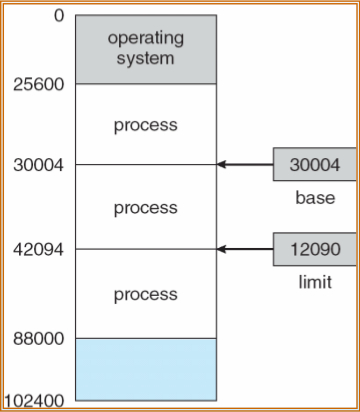
\includegraphics[scale=0.4]{images/memory_management/base_limit_regs.jpg}
\caption{Base and limit registers}
\end{figure}

Address biding of instructions and data to memory addresses can happen at three different stages:

\begin{itemize}
\item \textbf{Compile time}: If memory location is known a priori, \emph{absolute code} can be generated which must be recompiled if starting location changes;
\item \textbf{Load time}: If memory location is not known at compile time, \emph{relocatable code} must be generate;
\item \textbf{Execution time}: If the process can be moved during its execution from one memory to another, binding is delayed until run time and hardware support is needed for address mapping.
\end{itemize}

\begin{figure}[hbtp]
\centering
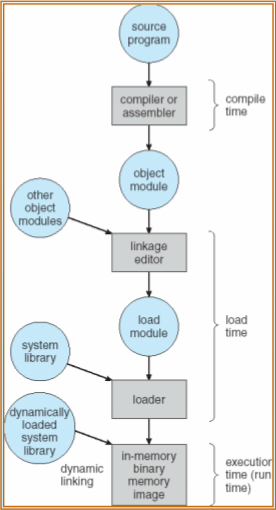
\includegraphics[scale=0.6]{images/memory_management/multistep_processing.jpg}
\caption{Multistep processing}
\end{figure}

Old CPUs generated ``static'' programs with pre-defined space and starting address, while modern CPUs generate logical addresses, starting from 0, mapped by the loader and the kernel into physical ones. In fact, loader interacts with the kernel, knowing which part of the memory are free and where to locate the program.
Addresses are always logical contiguous but pages are located around the memory, therefore the design is more complicated but more flexible, too.

\begin{itemize}
\item \textbf{Logical addresses} or \textbf{virtual addresses} are generated by the CPU;
\item \textbf{Physical addresses} are the addresses seen by the memory unit.
\end{itemize}
Logical and physical addresses are the same in compile time and load time address binding schemes; logical and physical addresses differ in execution time address binding scheme.

\subsection*{Memory management unit}
\emph{Memory management unit} is the hardware device responsible of mapping a virtual address into a physical one. The value in the \emph{relocation register} is added to every address generated by a user process at the time it is sent to memory. User programs deal with logical address, never with real physical addresses.

\begin{figure}[hbtp]
\centering
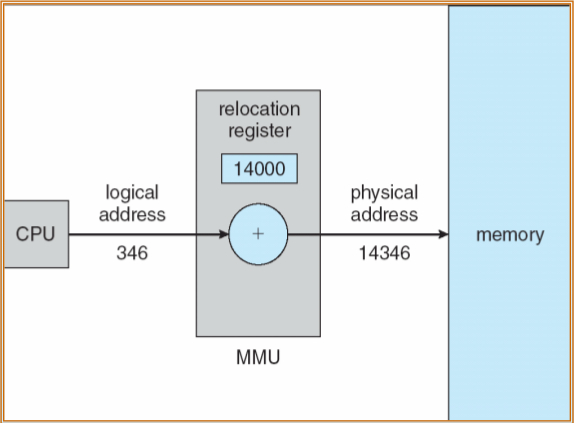
\includegraphics[scale=0.35]{images/memory_management/relocation_register.jpg}
\caption{Relocation register. From logical to physical address}
\end{figure}

\textbf{Dynamic loading} permits to load a routine on need. It is useful when large amounts of code are needed to handle infrequently occurring cases. In fact, an unused routine is never loaded, leading to a better memory-space utilization. No special support from the operating system is required, because it is implemented through program design.

\textbf{Dynamic linking} permits to postpone linking until execution time. A small piece of code, \emph{stub}, is used to locate the appropriate memory-resident library routine. Stub replaces itself with the address of the routine and executes the routine. Operating system needs to check if the routine is in the process' memory addresses. It is particularly useful for libraries.

\paragraph{Swapping}
A process can be temporarily swapped out of memory to a backing store and then brought back into memory to continue its execution. \emph{Backing store} is a fast disk large enough to accommodate copies of all memory images for all users, which must provide direct access to these memory images. The system maintains a \textbf{ready queue} of ready-to-run processes which have memory images on disk. \emph{Roll out, roll in} is a swapping variant used for priority-based scheduling algorithms: lower-priority process is swapped out so higher-priority process can be loaded and executed.

Major part of swap time is transfer time and the total transfer time is directly proportional to the amount of swapped memory.

\section{Contiguous allocation}
Usually, main memory is divided into two partitions:

\begin{itemize}
\item Resident operating system, usually held in low memory with interrupt vector;
\item User processes held in high memory.
\end{itemize}
Relocation registers are used to protect user processes from each other, and from changing operating system code and data. Memory management unit dynamically maps logical addresses.

When a process arrives, it is allocated memory from a hole\footnote{Block of available memory. Holes of various size are scattered throughout memory.} large enough to accommodate it. Operating system maintains information about allocated partitions and free partitions (holes). Different algorithms are available to satisfy a request from a list of free holes.

\begin{itemize}
\item \textbf{First-fit} allocates the first hole that is big enough;
\item \textbf{Best-fit} allocates the smallest hole that is big enough; it must scan the entire list, unless it is ordered by size, and produces the smallest leftover hole;
\item \textbf{Worst-fit} allocates the largest hole; it must scan the entire list too and produces the largest leftover hole.
\end{itemize}
First-fit and best-fit are better than worst-fit in terms of speed and storage utilization.

\paragraph{Fragmentation}
\begin{itemize}
\item \textbf{External Fragmentation}: total memory space exists to satisfy a request, but it is not contiguous;
\item \textbf{Internal Fragmentation}: allocated memory may be slightly larger than requested memory; this size difference is memory internal to a partition but not being used.
\end{itemize}
External fragmentation can be reduced by \emph{compaction} which is possible only if relocation is dynamic, it is done at execution time and implies to shuffle memory contents to place all free memory together in one large block.

\section{Paging}
Physical memory is divided into fixed-size blocks called \textbf{frames} and logical memory is divided into blocks of the same size called \textbf{pages}. In this way, logical address space of a process can be \emph{non-contiguous} and a process can be allocated in physical memory whenever the latter is available.

Each address generated by the CPU is divided into:
\begin{itemize}
\item \textbf{Page number}: used as an index into a \emph{page table} which contains base address of each page in physical memory;
\item \textbf{Page offset}: combined with base address to define the physical memory address that is sent to the memory unit.
\end{itemize}

\paragraph{Page table} \emph{Page table} is kept in main memory, identified by \textbf{Page table base register (PTBR)} pointing to the page table and \textbf{Page table length register (PRLR)} indicating size of the page table.

In this scheme, every access requires two memory accesses, the first one for the page table and the second one for the data/instruction. The two memory access problem can be solved by means of a special fast-lookup hardware cache called \emph{associative memory} or \textbf{translation look-aside buffer (TLB)}. An associative memory provides an address given a content, i.e.,\@ the opposite behavior with respect to a canonical memory.

\begin{figure}[hbtp]
\centering
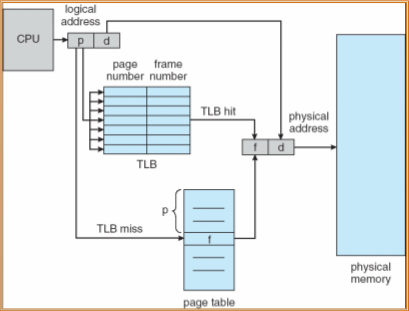
\includegraphics[scale=0.6]{images/memory_management/address_generation_tlb.jpg}
\caption{Address generation with TLB}
\end{figure}

Being $\epsilon$ the time for associative lookup, $t$  the cycle time and $\alpha$ the hit ratio, the \textbf{Effective Access Time} is calculated as $\text{EAT} = (t + \epsilon) \alpha + (2 t + \epsilon)(1 - \alpha)$

\paragraph{Memory protection} Memory protection is implemented by associating a protection bit with each frame. A \emph{valid-invalid bit} is attached to each entry in the page table:

\begin{itemize}
\item \textbf{Valid} indicates that the associated page is in the process' logical address space, and it is therefore a legal page;
\item \textbf{Invalid} indicates that the page is not in the process' logical address space.
\end{itemize}
TLB is an hardware structure and therefore shared. Hence, it has to be rebuilt on context switch.

One copy of read-only code can be shared among processes (i.e.,\@ text editors, compilers, window systems). Shared code must appear in the same location in the logical address space of all processes.

On the other hand, each process keeps a separate copy of the code and data. Pages for the private code and data can appear anywhere in the logical address space. Page table is inherited by a child process, in fact parent and child processes execute the same code and share the initial status. A new frame will be allocated by the process if it changes some variable content.

\subsection{Structure of the page table}
Having $n$ bits to store the page number, in kernel memory it is needed to have $2^n$ entries to store the page table.
\paragraph{Hierarchical Page Table} \emph{Hierarchical Page Table} breaks up the logical address space into multiple page tables. A simple technique is a two-level page table.

For example, a logical address on 32-bit machine with 1K page size is divided into:
\begin{itemize}
\item a page number consisting of 22 bits;
\item a page offset consisting of 10 bits.
\end{itemize}
Since the page table is paged, the page number is further divided into
\begin{itemize}
\item a 12-bit page number;
\item a 10-bit page offset.
\end{itemize}

\begin{figure}[hbtp]
\centering
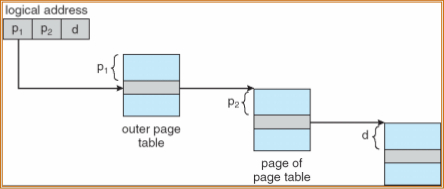
\includegraphics[scale=0.4]{images/memory_management/two_levels_pagetable.jpg}
\caption{Two levels page table}
\end{figure}

\paragraph{Hashed Page Table}
\emph{Hashed Page Table} is common in address space larger than 32 bits. The virtual page number is hashed into a page table containing a chain of elements hashing to the same location. Virtual page numbers are compared in this chain searching for a match and, if a match is found, the corresponding physical frame is extracted.

\begin{figure}[hbtp]
\centering
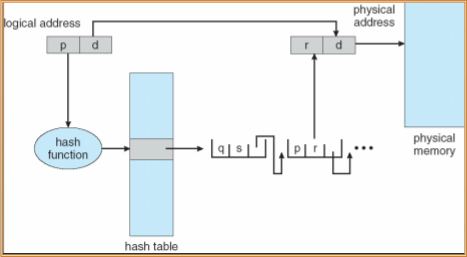
\includegraphics[scale=0.4]{images/memory_management/hashed_pagetable.jpg}
\caption{Hashed page table}
\end{figure}

\paragraph{Inverted Page Table}
\emph{Inverted Page Table} contains one entry for each real page memory. Each entry consists of the virtual address of the page stored in the real memory location, with information about the process which owns that page. This solution decreases the amount of needed memory to store each page table, but increases time needed to search the table when a page reference occurs.

\begin{figure}[hbtp]
\centering
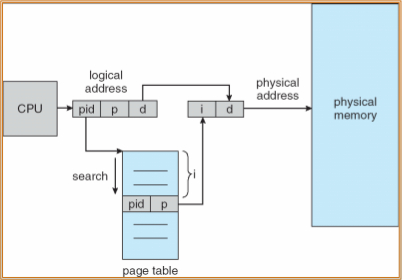
\includegraphics[scale=0.4]{images/memory_management/inverted_pagetable.jpg}
\caption{Inverted page table}
\end{figure}

\section{Segmentation}
\emph{Segmentation} is a memory management scheme which supports user view of memory. In fact, a program is a collection of segments\footnote{A segment is a logical unit containing homogeneous data with a variable size.}. Logically, an address consists of a two tuple composed by segment number and offset.

Segment table is identified by a \textbf{Segment table base register (STBR)}  pointing to the segment table's location in memory and \textbf{Segment table length register (STLR)} indicating the number of segments used by a program. Segment table maps two-dimensional physical addresses; each table entry has:
\begin{itemize}
\item \textbf{Base} containing the starting physical address where the segment resides in memory;
\item \textbf{Limit} specifying the length of the segment.
\end{itemize}

Protection is ensured associating a validation bit and read/write/execute privileges to each entry in segment table. Since segments vary in length, memory allocation is a dynamic storage allocation problem.

\section*{Memory mapping}
Instruction \texttt{mmap} allocates some memory for a file. It is useful if the file has to be read in a non-sequential way. In this way, file is seen as a memory array and the programmer does not care about reading or moving on the file because it is transparently done by the kernel.
Library \texttt{sys/mman.h} contains \texttt{mmap} function:
\newline
\texttt{void *mmap(void *addr, size\_t len, int prot, int flags, \\ int fd, off\_t off)}

It maps \texttt{len} bytes starting at offset \texttt{off} from the file specified by the file descriptor \texttt{fd} into the caller's address space and it returns the actual place where the object is mapped. \texttt{addr} is a hint only where to allocate the file, and is usually specified as 0 (\texttt{NULL}).

\texttt{prot} describes the desired memory protection as the bitwise or of \texttt{PROT\_READ}, \texttt{PROT\_WRITE} and \texttt{PROT\_EXEC}.

\texttt{FLAGS} is the bitwise or of
\begin{itemize}
\item \texttt{MAP\_SHARED}: any update made to the mapped region will be global, i.e.,\@ it will be seen by any other process (common option);
\item \texttt{MAP\_PRIVATE}: updates will be kept private to each process, copy on write;
\item Many other options on Linux.
\end{itemize}